

\section{Площадь круга и его частей}

\paragraph{}\label{1938/262}
\so{Лемма}.
\textbf{\emph{При неограниченном увеличении $\bm{n}$, сторона правильного вписанного $\bm{n}$-угольника делается как угодно малой.}}

Пусть $p_n$ есть периметр правильного вписанного $n$-угольника;
тогда длина одной его стороны выразится дробью $\frac {p_n}n$.
При неограниченном увеличении $n$ знаменатель этой дроби будет, очевидно, возрастать неограниченно, а числитель, то есть $p_n$, хотя и может возрастать, но не беспредельно,
так как периметр всякого вписанного выпуклого многоугольника всегда остаётся меньшим периметра любого описанного многоугольника.

Если же в какой-нибудь дроби знаменатель неограниченно возрастает, а числитель остаётся меньше некоторой постоянной величины, то дробь эта может сделаться как угодно малой.
Значит, то же самое можно сказать о стороне правильного вписанного $n$-угольника:
при неограниченном $n$ она может сделаться как угодно малой.

\begin{wrapfigure}[12]{r}{36mm}
\vskip-8mm
\centering
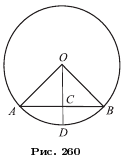
\includegraphics{mppics/ris-260}
\caption{}\label{1938/ris-260}
\end{wrapfigure}

\paragraph{}\label{1938/263}
\mbox{\so{Следствие}.}
Пусть $AB$ (рис. \ref{1938/ris-260}) есть сторона правильного вписанного многоугольника, $OA$ — радиус и $OC$ — апофема.
Из $\triangle OAC$ находим (§~\ref{1938/50}):
\[OA-OC<AC,\]
то есть
\[AO-OC<\tfrac12 AB.\]
Но при увеличении $n$, сторона правильного вписанного $n$-угольника, как мы сейчас доказали, может сделаться как угодно малой;
значит, то же самое можно сказать и о разности $OA-OC$.



Таким образом, \emph{при неограниченном увеличении $n$, разность между радиусом и апофемой правильного вписанного $n$-угольника может сделаться как угодно малой}.
Это же можно высказать другими словами так: 
\emph{предел, к которому стремится апофема $a_n$ правильного вписанного $n$-угольника, есть радиус.}



\paragraph{}\label{1914/230}
\so{Лемма}.
\textbf{\emph{Разность между площадью правильного $\bm{n}$-угольника, описанного около круга, и площадью правильного $\bm{n}$-угольника, вписанного в тот же
круг, стремится к нулю при неограниченном увеличении $\bm{n}$.}}

Впишем в окружность (рис. \ref{1914/ris-292}) и опишем около неё по правильному $n$-угольнику (на чертеже изображены $6$-угольники).
Пусть $R$ будет радиус круга, $a_n$ — апофема вписанного $n$-угольника, $q_n$ его площадь и $Q_n$ — площадь описанного $n$-угольника.
Тогда (§~\ref{1938/260})
\[\frac {Q_n}{q_n}=\frac{R^2}{a_n^2}\]

\begin{wrapfigure}[12]{r}{30mm}
\centering
\includegraphics{mppics/ris-1914-292}
\caption{}\label{1914/ris-292}
\end{wrapfigure}
\noindent
и следовательно 
\[\frac {Q_n-q_n}{q_n}=\frac{R^2-a_n^2}{a_n^2}.\]
Откуда
\[(Q_n-q_n)a_n^2=q_n(R^2-a_n^2)\]
или
\[(Q_n-q_n)a_n^2=q_n(R+a_n)(R-a_n).\]

При неограниченном увеличении $n$, разность $R-a_n$ стремится к нулю (§~\ref{1938/263}).
Сомножитель $q_n$ остаётся ограниченным, так как площадь вписанного многоугольника меньше площади любого описанного.  
Сомножитель $R+a_n$ всегда остаётся меньше $R+R$.
Вследствие этого правая часть последнего равенства (а значит и левая его часть),
при неограниченном увеличении $n$, стремится к нулю.

Заметим, что сомножитель $a_n^2$ в левой части возрастает при увеличении $n$ (§~\ref{1938/110}).
Значит левая часть может стремиться к нулю только тогда, когда другой сомножитель $Q_n-q_n$ стремится к нулю.
То есть разница площадей описанного и вписанного $n$-угольников стремится к нулю.

\paragraph{}\label{1914/231}
\so{Замечание}.
Таким же путём мы можем доказать, что \emph{разность между периметром описанного и
периметром вписанного правильного $n$-угольника, при неограниченном увеличении $n$, стремится к нулю.}

Действительно, если периметры правильных $n$-угольников, описанного и вписанного, обозначены буквами $P_n$ и $p_n$, то (Следствие в §~\ref{1938/218}):
\[\frac {P_n}{p_n}=\frac R{a_n}.\]
Откуда
\[\frac{P_n-p_n}{p_n}=\frac{R-a_n}{a_n},\]
и следовательно
\[(P_n-p_n)a_n=(R-a_n)p_n.\]

При неограниченном увеличении $n$ правая часть последнего равенства (а следовательно, и его левая часть) стремится к нулю, так как множитель $R-a_n$, по доказанному, стремится к нулю, а множитель $p_n$ остаётся ограниченным (так как периметр вписанного многоугольника не превосходит периметр любого описанного).
Но левая часть равенства, представляя собою произведение, в котором сомножитель $a_n$ увеличивается с ростом $n$, может стремиться к нулю только тогда, когда его другой сомножитель  стремится к нулю;
а этот сомножитель и есть разность периметров $P_n$ и $p_n$.

\paragraph{}\label{1914/232} \so{Теорема}. \textbf{\emph{Площадь круга есть oбщий предел площадей правильных вписанных в этот круг и описанных около него $\bm{n}$-угольников при неограниченном возрастании $\bm{n}$.}}

Пусть около круга, площадь которого мы обозначим $K$, описан правильный $n$-угольник и в него вписан правильный $n$-угольник (рис. \ref{1914/ris-292}).
Обозначим площадь первого $Q_n$ а площадь второго $q_n$.
При увеличении $n$, величины $Q_n$ и $q_n$ меняются, тогда как величина $K$ остаётся неизменной.
Требуется доказать, что при неограниченном увеличении $n$ величины $Q_n$ и $q_n$ стремятся к одному
и тому же пределу, а именно к площади $K$.

Заметим, что для любого $n$, выполняется неравенство 
\[Q_n>K>q_n\]
и потому каждая из двух разностей: 
$Q_n-K$ и $K-q_n$ всегда меньше разности $Q_n-q_n$.
Но при неограниченном увеличении $n$ разность $Q_n-q_n$ стремится к нулю (§~\ref{1914/230}).
Следовательно, при этом каждая из меньших разностей: $Q_n-K$ и $K-q_n$ и подавно стремится к нулю;
а это, согласно определению предела, означает, что $K$ является общим пределом для $Q_n$ и $q_n$.

\paragraph{}\label{1914/233} \so{Замечание}.
Можно также утверждать, что \emph{длина окружности есть общий предел периметров правильных вписанных в эту окружность и описанных около неё $n$-угольников при неограниченном увеличении $n$}.
Действительно, из того обстоятельства, что разность $P_n-p_n$ стремится к нулю (§~\ref{1914/231}), надо заключить, что периметры $P_n$ и $p_n$ могут стремиться только к одному и тому же пределу;
но предел $p_n$ есть то, что принимается за длину окружности;
значит, и предел $P_n$ равен длине окружности.

\paragraph{Площадь круга.}\label{1938/264}\ 
Впишем в круг, радиус которого обозначим $R$, какой-нибудь правильный $n$-угольник.
Пусть
\begin{align*}
\text{площадь}\quad&\text{этого многоугольника будет}&&q_n,
\\
\text{периметр}\quad&\text{—\textquotedbl—\qquad\quad —\textquotedbl—\qquad\quad —\textquotedbl—}&&p_n,
\\
\text{апофема}\quad&\text{—\textquotedbl—\qquad\quad —\textquotedbl—\qquad\quad —\textquotedbl—}&&a_n.
\end{align*}


Мы видели (§~\ref{1938/252}, следствие), что между этими величинами есть такая зависимость.
\[q_n=\tfrac12p_n\cdot a_n.\]

Вообразим теперь, что $n$ неограниченно увеличивается.
Тогда периметр $p_n$ и апофема  $a_n$ (следовательно, и площадь $q_n$) будут меняться, причём периметр будет стремиться к пределу, принимаемому за длину окружности $C$, апофема будет стремиться к пределу, равному радиусу круга $R$.
Из этого следует, что площадь $n$-угольника будет стремиться к пределу, равному $\tfrac12 C\cdot R$.
Но согласно §~\ref{1914/232} этот предел и есть площадь круга.

{\sloppy
Таким образом, обозначив площадь круга буквой $K$, можем написать:
\[K=\tfrac12 C\cdot R\]
то есть \emph{\textbf{площадь круга равна половине произведения длины окружности на радиус.}}

}

Так как $C=2\pi R$, то
\[K=\tfrac12\cdot 2\pi  R\cdot R=\pi R^2,\]
то есть \emph{\textbf{площадь круга равна квадрату радиуса, умноженному на отношение длины окружности к диаметру.}}

\paragraph{}\label{1938/265}
\so{Следствие}.
\emph{Площади кругов относятся, как квадраты радиусов или диаметров.}

Действительно, если $K$ и $K_1$ будут площади двух кругов, а $R$ и $R_1$ — их радиусы, то
\[K=\pi R^2\]
и
\[K_1=\pi R_1^2,\]
откуда
\begin{align*}
\frac{K}{K_1}&=\frac{\pi R^2}{\pi R^2_1}=\frac{R^2}{R^2_1}=
\\
&=\frac{4R^2}{4R^2_1}=\frac{(2R)^2}{(2R_1)^2}.
\end{align*}


\paragraph{}\label{1938/266}
\so{Задача 1}.
\emph{Вычислить площадь круга, длина окружности которого равна 2 м.}

Для этого предварительно находим радиус $R$ из равенства.
\[2\pi R= 2.\]
откуда
\[R=\tfrac1\pi=0{,}3183\dots\]

Затем определим площадь круга.
\[K=\pi R^2=\pi(\tfrac1\pi)^2=\tfrac1\pi=0{,}3183\dots\text{м}^2.\]

\paragraph{}\label{1938/267}
\so{Задача 2}.
\emph{Построить квадрат, равновеликий данному кругу.}

Эта задача, известная под названием \so{квадратуры круга}, не может быть решена при помощи циркуля и линейки.
Действительно, если обозначим буквой $x$ сторону искомого квадрата, а буквой $R$ радиус круга, то получим уравнение:
\[x^2=\pi R^2.\]
откуда
\[\frac{\pi R}{x}=\frac{x}{R}\]
то есть
$x$ есть средняя пропорциональная между полуокружностью и радиусом.
Следовательно, если известен отрезок, длина которого равна длине полуокружности, то легко построить квадрат, равновеликий данному кругу, и обратно, если известна сторона квадрата, равновеликого кругу, то можно построить отрезок, равный по длине полуокружности.
Но с помощью циркуля и линейки нельзя построить отрезок, длина которого равнялась бы длине полуокружности (§~\ref{1938/238});
следовательно, нельзя в точности решить задачу о построении квадрата, равновеликого кругу.
Приближённое решение можно выполнить, если предварительно найти приближённую длину полуокружности и затем построить среднюю пропорциональную между отрезком этой длины и радиусом.

\paragraph{}\label{1938/268}
\mbox{\so{Теорема}.}
\textbf{\emph{Площадь сектора равна произведению длины его дуги на половину радиуса.}}

Пусть дуга $AB$ (рис.~\ref{1938/ris-261}) сектора $AOB$ содержит $n\degree$.
Очевидно, что площадь сектора, дуга которого содержит $1\degree$, составляет $\tfrac1{360}$ часть площади круга, то есть она равна $\frac{\pi R^2}{360}$.
Следовательно, площадь $S$ сектора, дуга которого содержит $n\degree$, равна:
\[S=\frac{\pi R^2}{360}\cdot n\degree=\frac{\pi R\cdot  n\degree}{180}\cdot \frac R2.\]

\begin{wrapfigure}{r}{35mm}
\vskip-4mm
\centering
\includegraphics{mppics/ris-261}
\caption{}\label{1938/ris-261}
\end{wrapfigure}

\noindent
Так как дробь $\frac{\pi R n\degree}{180}$ выражает длину дуги $AB$ (§~\ref{1938/239}), то, обозначив
её буквой $s$, получим:
\[S=s\cdot \frac R2.\]

Заметим также, что если $\alpha$ угловая мера угла $AOB$ выраженная в радианах то $s=\alpha\cdot R$ (§~\ref{extra/radians}) и значит 
\[S=\frac{\alpha\cdot R^2}2.\]

\medskip
\mbox{\so{Замечание}.}
Строго говоря, предложенное рассуждение доказывает формулу
\[S=s\cdot \frac R2\]
только при целом значении $n$.
Аналогичным способом можно установить равенства в случае если угол $AOB$ имеет общую меру с полным углом.

Верность этого равенства для произвольных секторов доказывается аналогично лемме в §~\ref{1938/159};
то есть требуется предъявить произвольно близкие приближения для $S$ с недостатком и избытком между которыми лежит значение $s\cdot \frac R2$.

%!!! добавил замечание
{\sloppy

\paragraph{Площадь сегмента.}\label{1938/269}
Для нахождения площади сегмента, ограниченного дугой $s$ и хордой $AB$ (рис.~\ref{1938/ris-261}), надо отдельно вычислить площадь сектора $AOB$ и площадь треугольника $AOB$ и из первой вычесть вторую.

}

Впрочем, когда градусное измерение дуги $s$ невелико, площадь сегмента можно вычислять по следующей \so{приближённой} формуле (мы её приводим без доказательства):
\[\text{площадь сегмента}~\approx\tfrac23bh.\eqno(1)\]
где $b$ есть основание сегмента (рис.~\ref{1938/ris-262}), а $h$ — его высота (обыкновенно называемая \rindex{стрелка сегмента}\textbf{стрелкой сегмента}). 
Иначе говоря, площадь сегмента на рис.~\ref{1938/ris-262} близка к площади прямоугольника на том же рисунке. 

\begin{figure}[h]
\centering
\includegraphics{mppics/ris-262}
\caption{}\label{1938/ris-262}
\end{figure}

Доказано, что погрешность результата вычисления, получаемого по этой приближённой формуле, тем меньше, чем меньше отношение $\tfrac hb$;
так, если $h<\tfrac19b$ (что бывает тогда, когда дуга $s$ содержит меньше $50\degree$), то погрешность оказывается меньше 1\% площади.
Более точные результаты даёт более сложная формула.
\[\text{площадь сегмента}~\approx\tfrac23bh+\frac{h^3}{2b}.\eqno(2)\]


\subsection*{Упражнения}

\begin{center}
\so{Доказать теоремы}
\end{center}

\begin{enumerate}
\item
В параллелограмме расстояния от любой точки диагонали до двух прилежащих сторон обратно пропорциональны этим сторонам.

\item
Площадь трапеции равна произведению одной из непараллельных сторон на перпендикуляр, опущенный из середины другой непараллельной стороны на первую.

\item
Два четырёхугольника равновелики, если у них равны соответственно диагонали и угол между ними.

\item
Если площади двух треугольников, прилежащих к основаниям трапеции и образуемых пересечением её диагоналей, равны соответственно $p^2$ и $q^2$, то площадь всей трапеции равна $(p+q)^2$.

\item
Площадь правильного вписанного шестиугольника равна $\tfrac34$ площади правильного описанного шестиугольника.

\item
В четырёхугольнике $ABCD$ через середину диагонали $BD$ проведена прямая, параллельная другой диагонали $AC$.
Эта прямая пересекает сторону $AD$ в точке $E$.
Доказать, что отрезок $CE$ делит четырёхугольник пополам.

\item
Если медианы треугольника взять за стороны другого треугольника, то площадь последнего равна площади первого.

\item
В круге с центром $O$ проведена хорда $AB$.
На радиусе $OA$, как на диаметре, описана окружность.
Доказать, что площади двух сегментов, отсекаемых хордой $AB$ от обоих кругов, относятся, как 4:1.


\end{enumerate}

\begin{center}
\so{Задачи на вычисление}
\end{center}

\begin{enumerate}[resume]


\item
Вычислить площадь прямоугольной трапеции, у которой один из углов равен $60\degree$, зная или оба основания, или одно основание и высоту, или одно основание и боковую сторону, наклонную к основанию.

\item
Даны основания трапеции $B$ и $b$ и её высота Н.
Вычислить высоту треугольника, образованного продолжением непараллельных сторон трапеции до взаимного пересечения.

\item
В треугольник вписан другой треугольник, вершины которого делят пополам стороны первого треугольника;
в другой треугольник вписан подобным же образом третий;
в третий — четвёртый и~т.~д.
неограниченно.
Найти предел суммы площадей этих треугольников.

\item
По трём данным сторонам $a$, $b$ и $c$ треугольника вычислить радиус $r$ круга, вписанного в этот треугольник.

\smallskip
\so{Указание}.
Если $S$ есть площадь треугольника, то легко усмотреть, что
\[S=\tfrac12 ar+\tfrac12 br+\tfrac12 cr=pr,\]
где $p$ означает полупериметр треугольника.
С другой стороны, площадь $S$ выражается формулой Герона (§~\ref{1938/256}).
Отсюда можно получить формулу для $r$.


\item
Вычислить стрелку (высоту) и площадь сегмента в зависимости от радиуса $r$ круга, если центральный угол, соответствующий сегменту, содержит $60\degree$.
Вычисление это произвести тремя способами:
1) посредством вычитания из площади сектора площади треугольника;
2) по первой сокращённой формуле, указанной в §~\ref{1938/269};
3) по второй сокращённой формуле, указанной там же.
Сравните результаты вычисления друг с другом с целью определить абсолютную и относительную погрешности приближённых результатов.

\smallskip
\so{Решение}.
\[b=r;\]
\[h=r-\tfrac12 r\sqrt3=\tfrac12 r(2-\sqrt3)\approx 0{,}1340\cdot r;\]

1) площадь $p_1=\frac{\pi r^2}{6}-\frac{r^2\sqrt3}{4}\approx 0{,}0906\cdot r^2$;

2) площадь $p_2\approx \tfrac23 bh=\tfrac23\cdot r\cdot 0{,}1340\cdot r=0{,}0893\cdot r^2$;

3) площадь $p_3\approx \tfrac23 bh+\frac{h^3}{2b}=0{,}0893r^2+0{,}0012r^2=0{,}0905\cdot r^2$.

Абсолютная погрешность.
\[\text{для площади}~p_2 \approx 0{,}0906\cdot r^2 - 0{,}0893\cdot r^2 = 0{,}0013\cdot r^2;\]
\[\text{для площади}~p_3 \approx 0{,}0906\cdot r^2 - 0{,}0905\cdot r^2 = 0{,}0001\cdot r^2.\]
Относительная погрешность (то есть отношение абсолютной погрешности к измеряемой величине):
\[\text{для площади}~p_2 = \frac{p_1-p_2}{p_1}\approx\frac{0{,}0013r^2}{0{,}0906r^2}\approx0{,}014 = 1{,}4\%;\]
\[\text{для площади}~p_3 = \frac{p_1-p_3}{p_1}\approx\frac{0{,}0001r^2}{0{,}0906r^2}\approx0{,}001 = 0{,}1\%;\]
Таким образом, результат, вычисленный по первой приближённой формуле, меньше истинного результата (приблизительно) на $1{,}4\%$, а результат, вычисленный по второй приближённой формуле, меньше истинного на $0{,}1\%$.

\item
1) Зная основание $b$ сегмента и высоту его (стрелку) $k$, вычислить радиус $r$ круга.

\smallskip
\so{Указание}.
Из прямоугольного треугольника, у которого гипотенуза есть $r$, один катет $\frac b2$, а другой $r-h$, находим уравнение:
\[(\tfrac b2)^2+(r-h)^2=r^2\]
из которого легко определить $r$.

2) Вычислить диаметр круга, если известно, что при основании сегмента, равном $67{,}2$ см, стрелка его есть $12{,}8$ см (смотри предыдущее указание).

\smallskip
\so{Задачи на построение}

\item
Разделить треугольники прямыми, проходящими через его вершину, на три части, площади которых относятся, как $m\z:n:p$.

\item
Разделить треугольник на две равновеликие части прямой, проходящей через данную точку его стороны.

\item
Найти внутри треугольника такую точку, чтобы прямые, соединяющие её с вершинами треугольника, делили его на три равновеликие части.

\smallskip
\so{Указание}.
Разделим сторону $AC$ на $3$ равные части в точках $E$ и $E$.
Через $E$ проводим прямую, параллельную $AB$, и через $E$ — прямую, параллельную $BC$.
Точка пересечения этих прямых — искомая.

\item
То же — на три части в отношении $2:3:4$ (или вообще $m:n\z:p$).

\item
Разделить параллелограмм на три равновеликие части прямыми, исходящими из вершины его.

\item
Разделить параллелограмм на две части прямой, проходящей через данную точку на продолжении его стороны, так, чтобы их площади относились, как $m:n$. %Добавил «на продолжении его стороны» иначе указание работает не всегда!!!

\smallskip
\so{Указание}.
Среднюю линию параллелограмма разделить в отношении $m:n$ и точку деления соединить прямой с данной точкой.  

\item
Разделить параллелограмм на три равновеликие части прямыми, параллельными диагонали.

\item
Разделить площадь треугольника в среднем и крайнем отношении прямой, параллельной основанию.

\smallskip
\so{Указание}.
Решается приложением алгебры к геометрии.

\item
Разделить треугольник на три равновеликие части прямыми, перпендикулярными к основанию.

\item
Разделить круг на $2$, на $3,\dots$ равновеликие части концентрическими окружностями.

\item
Разделить трапецию на две равновеликие части прямой, параллельной основаниям.

\smallskip
\so{Указание}.
Продолжив непараллельные стороны до взаимного пересечения, взять за неизвестную величину расстояние от конца искомой линии до вершины треугольника;
составить пропорции, исходя из площадей подобных треугольников.

\item
Данный треугольник преобразовать в другой равновеликий прямоугольник с данным основанием.

\item
Построить квадрат, равновеликий $\tfrac23$ данного квадрата.

\item
Преобразовать квадрат в равновеликий прямоугольник, у которого сумма или разность $d$ двух смежных сторон дана.

\item
Построить круг, равновеликий кольцу, заключённому между двумя данными концентрическими окружностями.

\item
Построить треугольник, подобный одному и равновеликий другому из двух данных треугольников.

\item
Данный треугольник преобразовать в равновеликий равносторонний (посредством приложения алгебры к геометрии).

\item
В данный круг вписать прямоугольник с данной площадью $m$ (посредством приложения алгебры к геометрии).

\item
В данный треугольник вписать прямоугольник с данной площадью $m$ (приложением алгебры к геометрии; исследовать).

\end{enumerate}



